% 2009 年四川卷理科第 19 题：正方形 ABCD 与平面四边形 ABEF 所在平面互相垂直。
% 来源 PDF：普通高考/2009/2009四川理.pdf，SHA256 7f64be22c7f7c29a749b276635494972f962f91302ebc7506b55c9fae85a7406
% 原页：第 2 页（A3 三栏）第 1 栏中部，印刷页 558。
% 重绘依据：按原图取 A 左上、B 右上、C 右下、D 左下（斜投影平行四边形）；ABEF 为竖直平面，
%   E 在 A 正上方、F 在 A 的左上方，FA=FE；AB 被平面 ABEF 遮挡画虚线；
%   辅助线 EC、DB 与正方形边 AD、DC、CB 实线；P 为 DC 中点。第 (2) 问的 M 待求，图上不画。
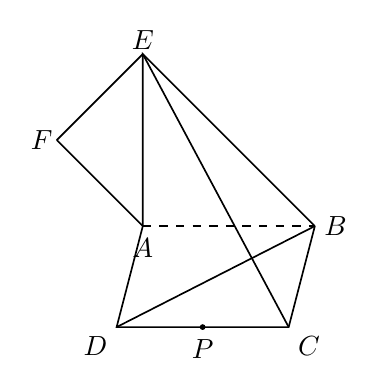
\begin{tikzpicture}[scale=0.95, semithick, every node/.style={inner sep=1.2pt}]
  \coordinate (A) at (0,0);
  \coordinate (B) at (2.3,0);
  \coordinate (C) at (1.95,-1.35);
  \coordinate (D) at (-0.35,-1.35);
  \coordinate (E) at (0,2.3);
  \coordinate (F) at (-1.15,1.15);
  \coordinate (P) at (0.8,-1.35);
  % 正方形（AB 被遮挡）
  \draw[dashed] (A) -- (B);
  \draw (B) -- (C) -- (D) -- (A);
  % 四边形 ABEF
  \draw (A) -- (E) -- (B);
  \draw (F) -- (A);
  \draw (F) -- (E);
  % 辅助线
  \draw (E) -- (C);
  \draw (D) -- (B);
  % 中点 P
  \fill (P) circle (1.1pt);
  \node[anchor=north] at ([yshift=-3pt]A) {$A$};
  \node[anchor=west] at ([xshift=2pt]B) {$B$};
  \node[anchor=north west] at ([xshift=2pt,yshift=-2pt]C) {$C$};
  \node[anchor=north east] at ([xshift=-2pt,yshift=-2pt]D) {$D$};
  \node[anchor=south] at (E) {$E$};
  \node[anchor=east] at (F) {$F$};
  \node[anchor=north] at ([yshift=-3pt]P) {$P$};
\end{tikzpicture}
